\documentclass{beamer}
\usepackage[size=a1,scale=1.8]{beamerposter}
\usetheme{LLT-poster}
\usecolortheme{ComingClean}
%\usecolortheme{ConspiciousCreep}
%\usecolortheme{Entrepreneur}

\usepackage[utf8]{inputenc}
\usepackage[T1]{fontenc}
%\usepackage{inconsolata}
\usepackage{zi4}
\usepackage{mathpazo}
\usepackage[scaled=0.95]{berasans}

\author[liantze@gmail.com]{Lim Lian Tze}
\title{Yet Another Beamer Poster Theme}
\institute{Multimedia University, Malaysia}
%\footimage{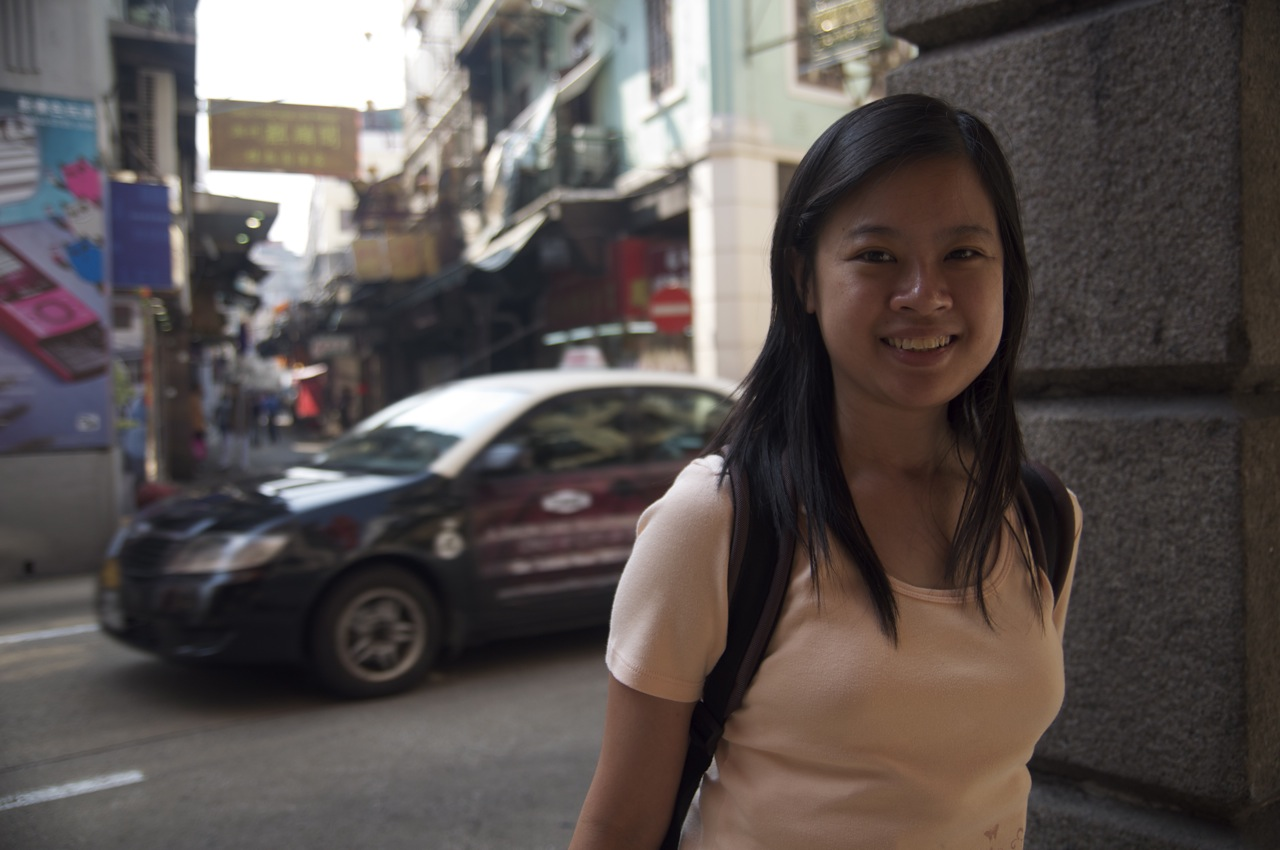
\includegraphics[height=15cm]{liantze}\hspace*{2em}}

\begin{document}
\begin{frame}\centering

\begin{columns}[T]
\begin{column}{.46\textwidth}
\begin{block}{This is a sample}
\begin{itemize}
\item One, two, pick up my shoe
\item Three, four, shut the door
\item Five, six, pick up sticks
\item Seven, eight, lay them straight
\item Nine, ten, a big fat hen
\end{itemize}
\end{block}
\end{column}
\begin{column}{.46\textwidth}
\begin{block}{This is another sample}
\begin{itemize}
\item Some maths material
\begin{align}
A &= U \times S \times V^T\\
\sigma &= \frac{x\times y}{\sqrt[3]{\alpha + \beta}}
\end{align}
\end{itemize}
\end{block}
\end{column}
\end{columns}

\end{frame}
\end{document}